\documentclass[11pt,a4paper]{article}
\usepackage[english]{babel}
\usepackage[letterpaper,top=2cm,bottom=2cm,left=3cm,right=3cm,marginparwidth=1.75cm]{geometry}
\usepackage{amsmath}
\usepackage{amsfonts} 
\usepackage{graphicx}
\usepackage{url}
\usepackage{float}

\DeclareMathOperator{\atantwo}{atan2}

\title{Image based trajectory determination of artificial satellites \\\large Preliminary outline on geometry, data acquisition and determination models}
\author{Frederic Heil\\
	\texttt{frederic.heil@hs-weingarten.de}}

\begin{document}
	\maketitle
	\section{Introduction}
	\label{sec:introduction}
	Image based trajectory determination of artificial satellites using ground based cameras is a multi-stage procedure that, in order to be implemented sucessfully, requires several problems to be solved. A thorough understanding of the underlying geometry and reference frames is needed. Once that has been established, methods for obtaining visual data can be defined, specifically for position and view vectors. These serve as an essential input for trajectory determinantion algorithms which will be used to determine the properties of a Keplarian orbit and its dedicated orbital plane.\newline
	The scope of this paper is limited to ground based observations, specifically systems using one or two cameas which are not supposed to change their location on earth for the process of imaging. No additional technologies, such as radar or laser measurements are to be used. Camera calibration in this context, specifically the process of determining view vectors, initially uses a star based calibration procedure, which limits the field-of-view range of cameras to certain values, which will be elaborated in section \ref{sec:determine_view_vecs}. Furthermore, the automated distinction between stars and satellites in measurement images could be considered as an additional problem to be solved, but is not part of the scope.\newline
	Trajectory-model-wise, the scope of this paper is limited to Keplarian orbits, which solve the 2-body problem with point masses. For the obsevable objects, namely artificial satellites, the main focus lies in the region of low earth orbit. Planet earth is the main gravitationally dominating force, observation arcs are rather short and because of this, more complicated orbital models are simply unfeasible, thus not part of the scope.


	\section{Geometry}
	\subsection{The Keplerian orbit}
	\label{sec:kepler_orbit}
	Geometrically, the shape of a Keplarian orbit can be described as an intersection between a plane and a cone, which carries some implications. Firstly, the shape of an orbit is either a circle, an ellipse, a parabola or a hyperbola. Secodly, as the intersection implies, the orbit lies within a plane. \cite{orbit_equation} \newline
	The current orbital radius $r$, which represents the current distance of an orbiting object (a satellite) from a gravitational center (planet earth) can be desrcibed with the following formula for circles and ellipses in a polar coordinate system, as provided by Weber \cite{elliptical_orbits} and modified to account for argument of periapsis $\omega$: 
	
	\begin{equation}\label{r_theta}
		r(\theta)=\frac{a(1-e^2)}{1+e\cdot\cos(\theta-\omega)}
	\end{equation}
	\noindent
	Hereby, $a$ represents the semi major axis of the orbit, which corresponds to the average distance between satellite and gravitational center. For elliptical orbits, this is just the average between the closest distance (periapsis $r_p$) and the furthest distance (apoapsis $r_a$), as illustrated in figure \ref{fig:parametric_ellipse}, stated below in equation \ref{semi_major_axis}:
	\begin{equation}\label{semi_major_axis}
		a = \frac{r_p + r_a}{2}
	\end{equation}
	\noindent
	The parameter $e$ represents the eccentricity, an inherent property of conic sections. For circles it is $e=0$, so that equation \ref{r_theta} collapses to $r(\theta)=a$. For ellipses it is $0 < e < 1$, for parabolas $e = 1$ and for hyperbolas $1 < e$. The parameter $\theta$ represents the so called true anomaly, which simply corrensponds to the parameter angle in a polar coordinate system. \cite{orbital_nomenclature} \newline
	The angle $\omega$ corrensponds to the argument of periapsis, which marks the closest distance (periapsis) in the polar coordinate system.\newline
	For hyperbolas, equation \ref{r_theta} is to be slightly modified, such that the sign of the dividend changes, which leads to: 
	\begin{equation}\label{r_theta_hyperbola}
		r(\theta)=\frac{-a(1-e^2)}{1+e\cdot\cos(\theta-\omega)} = \frac{a(e^2-1)}{1+e\cdot\cos(\theta-\omega)}
	\end{equation}
	\cite{hyperbolic_orbits} \newline
	This type of trajectories posess an asymptote, as visualized in \ref{fig:parametric_hyperbola}, which is never reached by the moving satellite. The asymptote, which the sattelite moves along, is the one with the gravitational center in its focal point. The semi major axis $a$ can also be defined by equation \ref{semi_major_axis}, however the apoapsis is located on the unreachable asymptote closest to the gravitational center, as illustrated in figure \ref{fig:parametric_hyperbola}.
	\newline
	As apparent from equation \ref{r_theta}, it does not hold up for an eccentricity value of $e = 1$ for parabolas. In case of $e = 1$ a modified equation is provided as follows:
	
	\begin{equation}\label{r_theta_parabolic}
		r(\theta)=\frac{p}{1+\cos(\theta-\omega)}
	\end{equation}
	\noindent
	Hereby $p$ corresponds to a constant value, so that $\frac{p}{2}$ equates to the distance between gravitational center and periapsis. A semi major axis value $a$ can not be defined as there is no apoapsis for this type of trajectory. \cite{parabolic_orbits}\newline
	Equations \ref{r_theta}, \ref{r_theta_hyperbola} and \ref{r_theta_parabolic} yield real numbers when plugging in concrete values for $\theta$. They can be expanded into parametric curves, which helps visualize the actual appearance of the different types of trajectories as follows:
	\begin{equation}
		\begin{aligned}
			r(\theta)=\frac{a(1-e^2)}{1+e\cdot\cos(\theta-\omega)} \cdot \begin{pmatrix}
				\cos(\theta) \\
				\sin(\theta)
			\end{pmatrix} \\
			r(\theta)=\frac{a(e^2-1)}{1+e\cdot\cos(\theta-\omega)} \cdot \begin{pmatrix}
				\cos(\theta) \\
				\sin(\theta)
			\end{pmatrix} \\
			r(\theta)=\frac{p}{1+\cos(\theta-\omega)} \cdot \begin{pmatrix}
				\cos(\theta) \\
				\sin(\theta)
			\end{pmatrix}
		\end{aligned}
	\end{equation}
	\noindent
	
	\begin{figure}[H]
		\centering
		\begin{minipage}{0.48\linewidth}
			\centering
			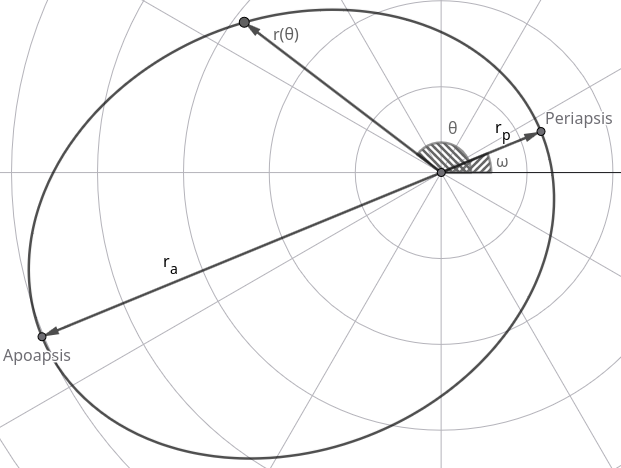
\includegraphics[width=\linewidth]{images/ellipse_parametric.png}
			\caption{Parametric curve of an elliptic obit.}
			\label{fig:parametric_ellipse}
		\end{minipage}
		\hfill
		\begin{minipage}{0.48\linewidth}
			\centering
			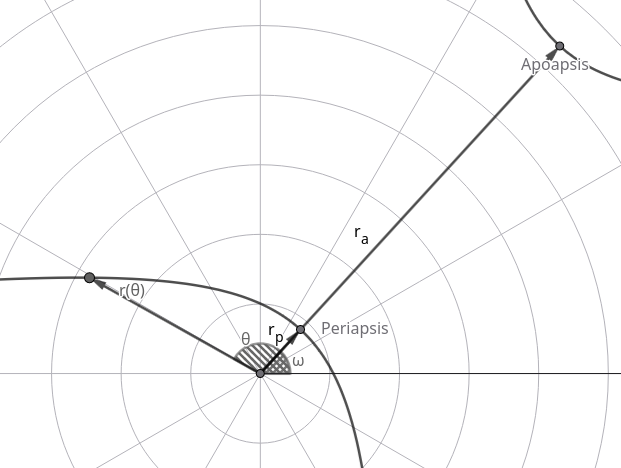
\includegraphics[width=\linewidth]{images/hyperbola_parametric.png}
			\caption{Parametric curve of a hyperbolic trajectory.}
			\label{fig:parametric_hyperbola}
		\end{minipage}
		
	\end{figure}
	\noindent
	This covers the different types of Keplarian trajectories as well as their properties in two dimensions.\newline
	Stated above, geometrically, each trajectory can be defined as an intersection between a cone and a plane in three dimensions. This leaves the property of the orbital plane to be defined. This plane always contains the point of the gravitational center. Also, the gravitational center shall be defined as the origin of the coordinate system, as elaborated below in section \ref{sec:reference_coordinate}.
	Hence, the plane can be sufficiently defined by a normal vector.
	
	\subsection{Reference coordinate system}
	\label{sec:reference_coordinate}
	The reference coordinate system of our choice is the Earth Centered Inertial (ECI) coordinate system. This coordinate system is aligned to planet earth but not fixed to its surface. The Z-axis is aligned to earth's rotation axis, while the X-Y-plane is aligned to earth's equatorial plane, as visualized below. Both X-, and Y-axes are fixed in reference to the background stars. Each position can be described by a vector in $\mathbb{R}^3$.
	
	\begin{figure}[H]
		\centering
		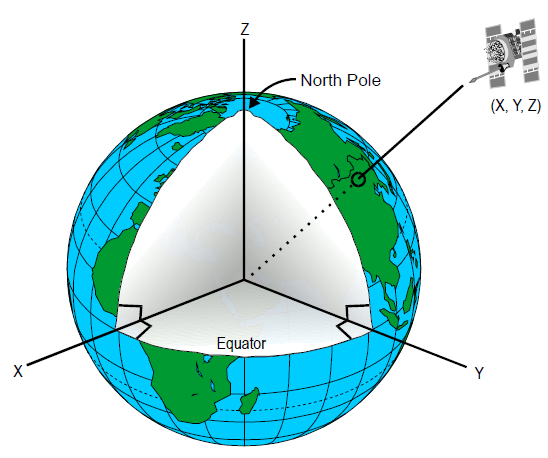
\includegraphics[width=0.45\linewidth]{images/Earth_Centered_Inertial_Coordinate_System.png}
		\caption{Earth Centered Inertial coordinate system aligned to planet earth. \cite{reference_frames}}
		\label{fig:eci}
	\end{figure}
	\noindent
	In this reference frame, when stationed at a fixed loction on planet earth, the position vector changes over time. This is different from the Earth Centered Earth Fixed (ECEF) coordinate system, which is fixed to earth's surface, such that position vectors in a fixed position do not change over time. \cite{reference_frames}
		
	\section{Data acquisition}
	\subsection{Earth bound camera based observation}
	\label{sec:eath_bound_observation}
	Before setting up mathematical models and implemanting trajectory determination algorithms, we need to take a look at what kind of data is readily available, what is unavailable (to be determined by algorithms later on) and how observed images look like. This serves as the basis on how we have to define models and what problems need to be solved. For this purpose, we define the geometric model of a stationary observer / camera on the surface of planet earth using the following figure:
	
	\begin{figure}[H]
		\centering
		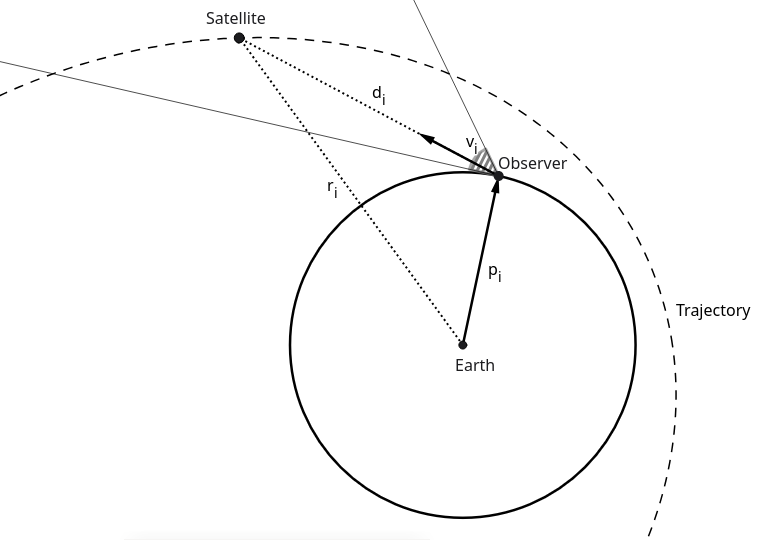
\includegraphics[width=0.8\linewidth]{images/knowns_and_unknowns.png}
		\caption{Initially known and unknown properties of earth bound camera based satellite observation depicted in a two dimensional represention.}
		\label{fig:knowns_and_unknowns}
	\end{figure}
	\noindent
	Hereby, all variables are annotated with an index $i$. That is, because these values change over time and are only valid for a certain time stamp $i$, which is a known property.\newline
	The first readily available propery apart from the time stamp is the position vector $p_i \in \mathbb{R}^3$, which describes the stationary position of the observer on planet earth in ECI coordinates. The determination of this property is elaborated in section \ref{sec:determination_position}.\newline
	Secondly, we have the view vector $v_i \in \mathbb{R}^3$. This vector marks the visual direction of the satellite as seen from the observer's position in ECI coordinates. The magnitude of this vector does not match the distance between the observer and the satellite, as this property is yet to be determined. Because of this, the value if the vector is normed to unit length.
	Further known or readily determinable properties are camera properties. For one, the camera's field of view is a fixed value. Moreover, the cameras alignment / rotation is readily determinable, so that each pixel can be assigned to a view vector $v_i$. The process of view vector determination and camera alignment is elaborated in section \ref{sec:determine_view_vecs}.\newline
	This sums up all readiliy available or readily determinable properties of earth bound camera based satellite observation. The unknown properties of this model comprise of the absolute position vector of the satellite $r_i \in \mathbb{R}^3$ and the distance vector $d_i \in \mathbb{R}^3$ which marks the distance between observer and satelitte, of which only the direction is known as $v_i$. The vectors are related to one another as they form the sum $r_i = p_i + d_i$. \newline
	Now, that available and unavailable parameters have been established, we can examine the visual data that is captured as images and what the appearance of satellites will be. \newline
	As visible from the ground, satellites appear as more or less bright dots similar to stars, even so that they may be observable to the naked eye. Their movement appears smoothly and their brightness does not change drastically, as they do not posess flashing lights like aircraft. They are illuminated by the sun, until they enter earth's shadow at whicht they become invisible. \cite{satellites_at_night}
	\begin{figure}[H]
		\centering
		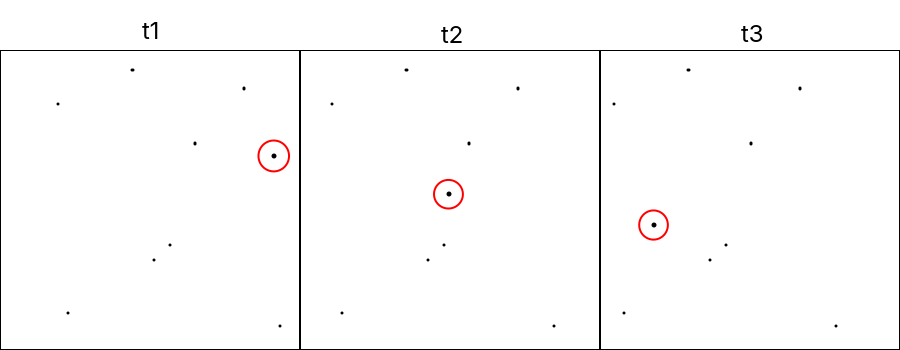
\includegraphics[width=0.8\linewidth]{images/s_captures_moved.png}
		\caption{Stars and a sattelite (encircled) are perceived as dots by cameras.}
		\label{fig:satelitte_appearance}
	\end{figure}
	\noindent
	Illustrated above in figure \ref{fig:satelitte_appearance} are three image frames, supposed to be taken at three time stamps $t_1$, $t_2$ and $t_3$ by a ground-fixed camera. In each frame, stars and a satellite (encircled) are visible. For one, the satellite would not be distinguishable from the background stars if it were not marked. Differentiation between satellites and stars may be automated, however we consider this issue not to be part of this research project.\newline
	Next up, there are two relevant types of apparent movenents visible in the image series. As planet earth rotates, background stars move slowly in the image frame. The apparent movement of the satellite is caused mainly by its inherent movement along its trajectory and marginally by the rotation of planet earth. \newline
	These aspects have to be factored in especially during camera alignment and view vector determination procedures.
	\subsection{Determination of position vectors}
	\label{sec:determination_position}
	As stated previously in section \ref{sec:eath_bound_observation}, the position vector $p_i$ in ECI coordinates is a readily available value. The actual vector values are initially unknown and have to be derived from known values of the observer. These known values are latitude, longitude and height on earth and the current time stamp. From these four values, the $p_i$ vector can be sufficiently derived.
	First of all, we have to factor in the shape of planet earth, which is ellipsoidal, rather than perfectly spherical. Sanz Subirana et. al. provide a set of equations to perform a transformation from latitude, longitude and height to a $\mathbb{R}^3$ vector in ECEF coordinates, which can be transformed to ECI coordinates later on.\newline
	As follows, we define latitude as $\varphi$, longitude as $\lambda$ and height above ellipsoid as $h$. Further known general values are earth's equatorial radius $a$ and polar radius $b$. The geometric context is illustrated in figure \ref{fig:cartesian_ellipsoidal} below:
	
	\begin{figure}[H]
		\centering
		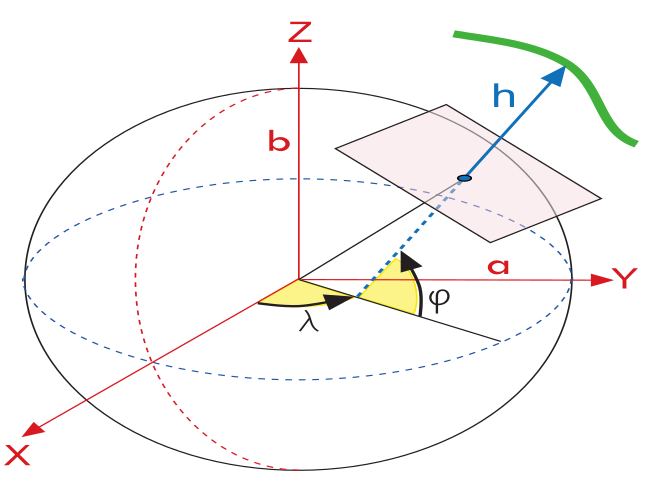
\includegraphics[width=0.5\linewidth]{images/cartesian_ellipsoidal.png}
		\caption{Cartesian and ellipsoidal coordinates on planet earth. \cite{esa_cartesian_ellipsoidal}}
		\label{fig:cartesian_ellipsoidal}
	\end{figure}
	\noindent
	As the shape of earth is ellipsoidal, an ellipse can be defined as a section of the ellipsoid along the Z-axis, for example in the YZ-plane. This ellipse, just as the orbital ellipses posesses an eccentricity $e$ which is defined as follows:
	\begin{equation}
		\label{ellipsoid_e}
		e^2=\frac{a^2 - b^2}{a^2}
	\end{equation}
	Using the value of $e$, the radius $N$ of the prime vertical is defined as follows:
	\begin{equation}
		\label{ellipsoid_N}
		N=\frac{a}{\sqrt{1-e^2\sin(\varphi)^2}}
	\end{equation}
	Using $e$, $N$ and the height value $h$, the components of position vector $p$ can now be sufficiently defined as:
	\begin{equation}
		\label{ellipsoid_p}
		p=
		\begin{pmatrix}
			p_x \\
			p_y \\
			p_z
		\end{pmatrix} = 
		\begin{pmatrix}
			(N+h)\cos(\varphi)\cos(\lambda) \\
			(N+h)\cos(\varphi)\sin(\lambda) \\
			((1-e^2)N+h)\sin(\varphi)
		\end{pmatrix}
	\end{equation}
	\cite{esa_cartesian_ellipsoidal}\newline
	In the ECEF coordinate system, the longitude value $\lambda$ is always fixed. In the ECI coordinate system, earth rotates around the Z-axis, as such that of the parameters latitude, longitude and height only longitude in reference to the ECI coordinate origin changes as time progresses. To determine longitude subject to time, Curtis provides a set of equations and a process to solve this issue. To elaborate the following process, some underlying geometric elements must be defined beforehand.
	
	\begin{figure}[H]
		\centering
		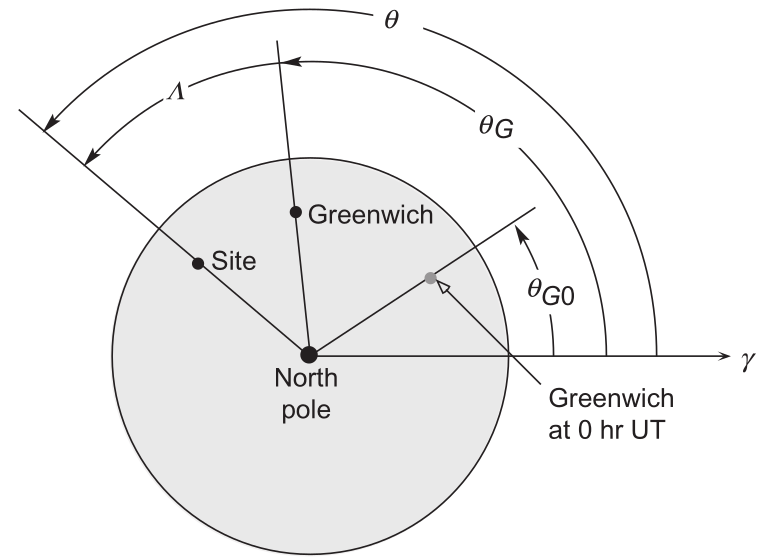
\includegraphics[width=0.47\linewidth]{images/siderial_time.png}
		\caption{Geometric context of ECI longitude subject to time.  \cite{curtis_siderial_time}}
		\label{fig:curtis_siderial_time}
	\end{figure}
	\noindent
	As illustrated above in figure \ref{fig:curtis_siderial_time}, the geometric context consists of several angles along the polar axis, which corresponds to the Z-axis in our ECI coordinate system, as illustrated in figure \ref{fig:eci}. The axis $\gamma$ corresponds to the X-axis. Time stamps in this context are defined as \emph{YYYY.MM.DD HH:MM:SS}, which consists of year, month, day, hours, minutes and seconds to date any observation in Universal Time (UT).\newline
	The first relevant value is $\theta_{G0}$, which corresponds to ECI longitude angle at which Greenwhich (hereby short for the prime meridian of the ECEF coordinate system) is located on any day at 0hr UT, meaning \emph{YYYY.MM.DD 00:00:00}. \newline
	Next up, we have $\theta_{G}$, the angular location of Greenwich at the time stamp of observation, meaning that hours, minutes and seconds in the time stamp are fully specified. \newline
	Finally we have $\Lambda$ and $\theta$ related by $\theta=\Lambda+\theta_{G}$, where $\Lambda$ describes the longitude angle between observer and Greenwich at time of observation and $\theta$ describes the longitude angle between observer and axis $\gamma$.
	To determine these values, specifically starting with $\theta_{G0}$, a complex process is required which consists of several steps, outlined below:
	\begin{enumerate}
		\item The determination of the current Julian day ($J_0$):\newline The current Julian day depicts the number of days since noon (UT) on January 1st, 4713 BC. For any given date within limitations, consisting of year (y), month (m) and day (d), the following formula applies:
		\begin{equation}
			J_0 = 367y - \left\lfloor
			\frac{7\left(y + \left\lfloor \frac{m+9}{12} \right\rfloor\right)}{4}
			\right\rfloor + \left\lfloor \frac{275m}{9}\right\rfloor + d + 1721013.5
		\end{equation}
		constrained to $1901 \leq y \leq 2099$, $1 \leq m \leq 12$ and $1 \leq d \leq 31$.
		
		\item The determination of $T_0$ in the J2000 epoch:\newline
		The J2000 Julian epoch starts noon (UT) on January 1st, 2000 and marks the number of days since the start of the Julian calendar, which is 2451545. This step consists of calculating the number of Julian centuries $T_0$ between the start of J2000 and the current observation date. This can be archieved with the following formula containing the result of the previous step:
		\begin{equation}
			T_0 = \frac{J_0-2451545}{36525}
		\end{equation}
		
		\item The determination of $\theta_{G0}$: \newline
		With the result $T_0$ of the previus step, we can now determine the angle $\theta_{G0}$ with the following polynomial, which yields the value in degrees:
		\begin{equation}
			\theta_{G0} = 100.4606184 + 36000.77004\cdot T_0 + 0.000387933\cdot T_0^2 -2.583(10^{-8})\cdot T_0^3
		\end{equation}
		
		\item The determination of $\theta_{G}$ and $\theta$:\newline
		Having calculated $\theta_{G0}$, we can now compute $\theta_{G}$ for any arbitrary time of the day using the following equation, which yields a degree value:
		\begin{equation}
			\theta_{G} = \theta_{G0} + 360.98564724^\circ\cdot\frac{UT[\mathrm{hr}]}{24[\mathrm{hr}]}
		\end{equation}
		Hereby $UT$ corresponds to the current time of the day as floating point number (e.g. the time value 09:41:22 corresponds to 9.68944 [hr]). The angular value slightly above 360° stems from the fact, that the rotation of earth against the background stars, a siderial rotation, is slightly shorter than 24 hours. With $\theta_{G}$ determined and known $\Lambda$ value, $\theta$ arised from the geometric context as $\theta=\Lambda+\theta_{G}$.
	\end{enumerate}
	\cite{curtis_siderial_time}
	\newpage\noindent
	Now, that $\theta$, the longitude of the observer in ECI coordinates at a specific time stamp $i$, has been determined, we can use the previously established equation \ref{ellipsoid_p} to determine the position vector. This can be done by inserting $\theta$ for $\lambda$ which yields the final result of $p_i$.
	
	\subsection{Determination of camera alignment and view vectors}
	\label{sec:determine_view_vecs}
	This section elaborates the determination of camera alignment and view vectors using a star based calibration procedure, as previously established. Hereby a view vector constitutes to the variable $v_i$ as explained in section \ref{sec:eath_bound_observation}. As for the camera alignment, we assume that any observer camera is fixed to the ground (as in fixed to the ECEF coordinate system) and pointing in a certain direction. Furthermore it may be rotated in such a way, that we initially can not deduct any view vectors (in ECI coordinates) from dots in an image.
	\begin{figure}[H]
		\centering
		\begin{minipage}{0.32\linewidth}
			\centering
			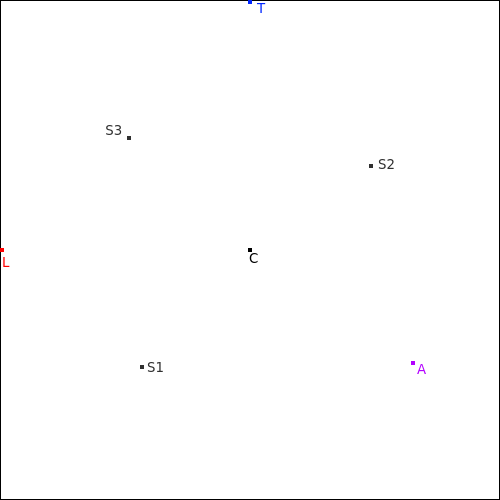
\includegraphics[
			width=\linewidth]{images/cam_calib.png}
			\caption{Calibration aspects of an image}
			\label{fig:cam_calib_blank}
		\end{minipage}
		\hfill
		\begin{minipage}{0.32\linewidth}
			\centering
			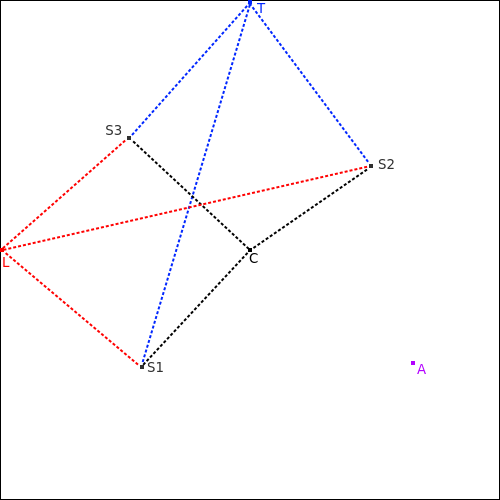
\includegraphics[width=\linewidth]{images/cam_calib_points.png}
			\caption{Determination of camera alignment}
			\label{fig:cam_calib_points}
		\end{minipage}
		\hfill
		\begin{minipage}{0.32\linewidth}
			\centering
			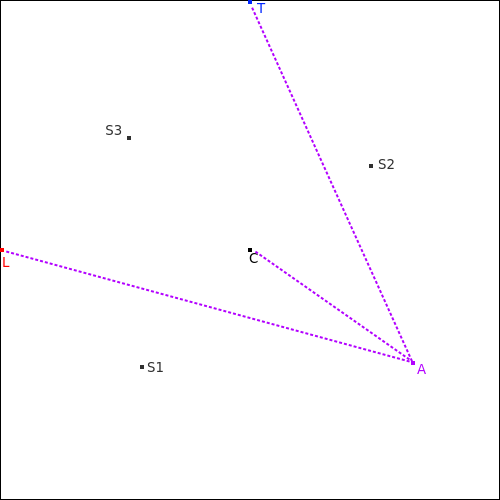
\includegraphics[width=\linewidth]{images/cam_calib_sat.png}
			\caption{Determination of the view vector}
			\label{fig:cam_calib_sat}
		\end{minipage}
	\end{figure}
	\noindent
	First, we need to determine alignment which constitutes to the calibration of the camera. Illustrated in figure \ref{fig:cam_calib_blank} are visual components of an image, taken at a certain time stamp, which are necessary for calibration. Within the image frame, we define three key points: $C$ (located in the center), $T$ (centered on the top edge) and $L$ (centered on the left edge). Visible within the image are dots, which correspond to at least three known stars ($S1$, $S2$ and $S3$) and (initially optional) the artificial satellite $A$. The assignment of three dots to actual known stars requires a star matching algorithm to be carried out. Such an algorithm has been established in a previous work \cite{self_localization_in_space} which constitutes to a modified version of the brightness independent 4-Star matching algorithm presented by Ying et. al. \cite{four_stars_algo}.\newline
	Once three stars have been identified, three view vectors (in ECI coordinates) $v_{S1}$, $v_{S2}$ and $v_{S3}$ can be assigned to the three dots $S1$, $S2$ and $S3$.\newline
	Figure \ref{fig:cam_calib_points} illustrates the triangulation of the key points $C$, $T$ and $L$, a process that yields three corresponding view vectors $v_C$, $v_T$ and $v_L$. To triangulate any pixel point $P$, as in to determine $v_P$, we have to determine the angular distances between the stars dots and $P$ first using the following formula:
	\begin{equation}
		\label{img_angular_dist}
		\gamma_i = \delta \cdot \frac{d_i}{w}= \delta \cdot \frac{|S_i-P|}{w}
	\end{equation}
	It is assumed that the image is rectilinear and square with a fixed pixel width $w$ and a corresponding agular diameter $\delta$. The value $\gamma_{i}$ represents the angular distance between a star point $S_i$ and $P$, whereas their pixel distance is expressed as $d_i$. These $\gamma$ values are to be determined between any $P$ and each of the three stars and are plugged in to the next equation:
	
	\begin{equation}
		\label{img_lgs}
		\begin{bmatrix}
			\text{---} & v_{S1} & \text{---} \\
			\text{---} & v_{S2} & \text{---} \\
			\text{---} & v_{S3} & \text{---}
		\end{bmatrix}\cdot
		\begin{bmatrix}
			v_P
		\end{bmatrix}=
		\begin{bmatrix}
			\cos(\gamma_{1}) \\
			\cos(\gamma_{2}) \\
			\cos(\gamma_{3}) \\
		\end{bmatrix}
	\end{equation}
	Solving this equation vor $v_P$ yields the corresponding vector value (in ECI coordinates) for any point $P$ on the image. \cite{self_localization_in_space}\newline
	If the artificial satellite $A$ is visible in the same image, $v_A$ can be determined similarly using equations \ref{img_angular_dist} and \ref{img_lgs} using the same process. A more generalized approach however is to determine $v_A$ of $A$ by triangulating it with the previously triangulated points $C$, $T$ and $L$, as shown in figure \ref{fig:cam_calib_sat}. Initially after calibration the satellite might not be visible in the camera's field of view, but at a later point in time. Stated previously, the camera is fixed to the ground, meaning that the observation frame moves as earth rotates. This means, that the determined image calibration vectors $v_C$, $v_T$ and $v_L$ which are fixed to the image also move with earth's rotation. Supposing that $v_C$, $v_T$ and $v_L$ have been determined at time stamp $t_0$, we can determine $v_C'$, $v_T'$ and $v_L'$ at $t_1$ using the following rotation angle and formula:
	
	\begin{equation}
		\label{vector_rotation}
		\begin{aligned}
			\alpha=360.98564724^\circ\cdot \frac{\varDelta t}{T_d}=360.98564724^\circ\cdot \frac{(t_1-t_0)[\mathrm{hr}]}{24[\mathrm{hr}]} \\
			v_P'=
			\begin{bmatrix}
				\cos(\alpha) & -\sin(\alpha) & 0 \\
				\sin(\alpha) & \cos(\alpha) & 0 \\
				0 & 0 & 1 \\
			\end{bmatrix}
			\cdot v_P
		\end{aligned}
	\end{equation}
	Stated previously in section \ref{sec:determination_position}, earth rotates slightly more than 360° in 24 hours relative to the ECI coordinate system. With the difference $t_1-t_0$ we obtain the rotation angle $\alpha$ at which the observer location rotates relative to the Z-axis. That angle can be applied to $v_P$ using a rotation matrix which rotates the vector around the Z-axis as well.\newline
	As the satellite dot shows up in a later image at $t_1$, we can now triangulate $v_A$ of $A$ using $v_C'$, $v_T'$ and $v_L'$ equivalently to the previously performed star calibration of $C$, $T$ and $L$.
	
	
	\section{Orbit determination models}
	\subsection{Parametric trajectory from angles and radii}
	\label{sec:parametric_trajectory}
	Previously, in section \ref{sec:kepler_orbit} we have established the Keplerian orbit. Elliptical and hyperbolic orbits can be described using equations \ref{r_theta} and \ref{r_theta_hyperbola}, characterized by $a$, $e$ and $\omega$. These equations differ from each other in the sign, but yield similar curves mirrored at the X-axis if equipped with the same values $a$, $e$ and $\omega$ otherwise. For this reason, equation \ref{r_theta} can also be used to model hyperbolic trajectories, the sign is simply flipped. If we allow negative values specifically for $a$ and $e$, this issue can be omitted and equation \ref{r_theta} can be used in the following to model both elliptical and hyperbolic trajectories.\newline
	We start off with three distinct measurements where three radii $r_i$ and three angles $\theta_i$ for $i \in \{1,2,3\}$ are known. Geometric context is given in figures \ref{fig:parametric_ellipse} and \ref{fig:parametric_hyperbola}. Going back to section \ref{sec:eath_bound_observation} we know that $r_i$ values are initially unknown. Their determination is an issue for upcoming sections.\newline
	We start the derivation process by plugging in radii and angular values into equation \ref{r_theta}, which yields a system of three equations for $i \in \{1,2,3\}$ structured as follows:
	
	\begin{equation}\label{derivation_basis}
		r_i=\frac{a(1-e^2)}{1+e\cdot\cos(\theta_i-\omega)}
	\end{equation}
	
	\noindent
	From this, we rearrange equation \ref{derivation_basis} to factor out $a$ subject to $e$ and $\omega$ as follows:
	
	\begin{equation*}
		r_i=\frac{a(1-e^2)}{1+e\cdot\cos(\theta_i-\omega)} \Leftrightarrow a=\frac{r_i(1+e\cdot\cos(\theta_i-\omega))}{1-e^2}
	\end{equation*}
	\begin{equation}\label{halbachse}
		\boxed{a=\frac{r_i(1+e\cdot\cos(\theta_i-\omega))}{1-e^2}}
	\end{equation}
	Next up, we obtain $e$ subject to $\omega$ by equating expression \ref{halbachse} with itself but with two different index values $i$ and $j$ with $j \in \{1,2,3\}$ and $i \neq j$ to use different radii and angles as follows:
	
	\begin{equation*}
		\begin{aligned}
			\frac{r_i(1+e\cdot\cos(\theta_i-\omega))}{1-e^2}=\frac{r_j(1+e\cdot\cos(\theta_j-\omega))}{1-e^2} \Leftrightarrow \\
			r_i+r_ie\cdot\cos(\theta_i-\omega)=r_j+r_je\cdot\cos(\theta_j-\omega) \Leftrightarrow \\
			r_i-r_j=e(r_j\cdot\cos(\theta_j-\omega)-r_i\cdot\cos(\theta_i-\omega))
		\end{aligned}
	\end{equation*}
	\noindent
	Some simplications can be applied:\newline $C_{ij}\cdot\cos(\alpha_{ij}-\omega) = r_j\cdot\cos(\theta_j-\omega)-r_i\cdot\cos(\theta_i-\omega)$ and \newline
	$\alpha_{ij}=\atantwo(B_{ij}, A_{ij})$ with \newline $C_{ij}=\sqrt{A_{ij}^2+B_{ij}^2}$ , $A_{ij}=\cos(\theta_j)r_j-\cos(\theta_i)r_i$ and $B_{ij}=\sin(\theta_j)r_j-\sin(\theta_i)r_i$.\newline
	Hence:
	\newline
	\begin{equation*}
		\begin{aligned}
			r_i-r_j=e(C_{ij}\cdot\cos(\alpha_{ij}-\omega)) \Leftrightarrow 
			\frac{r_i-r_j}{C_{ij}\cdot\cos(\alpha_{ij}-\omega)}=e
		\end{aligned}
	\end{equation*}
	\begin{equation}\label{excentritaet}
		\boxed{e=\frac{r_i-r_j}{C_{ij}\cdot\cos(\alpha_{ij}-\omega)}}
	\end{equation}
	\noindent
	Next up, we obtain $\omega$ by equating expression \ref{excentritaet} with itself with two different index pairs $ij$ and $ik$ with $k \in \{1,2,3\}$ and $i \neq j \neq k$ as follows:
	
	\begin{equation*}
		\begin{aligned}
			\frac{r_i-r_j}{C_{ij}\cdot\cos(\alpha_{ij}-\omega)}=\frac{r_i-r_k}{C_{ik}\cdot\cos(\alpha_{ik}-\omega)} \Leftrightarrow \\
			(r_i-r_j)\cdot(C_{ik}\cdot\cos(\alpha_{ik}-\omega))=(r_i-r_k)\cdot(C_{ij}\cdot\cos(\alpha_{ij}-\omega)) \Leftrightarrow \\
			\frac{C_{ik}(r_i-r_j)}{C_{ij}(r_i-r_k)}=\frac{\cos(\alpha_{ij}-\omega)}{\cos(\alpha_{ik}-\omega)}
		\end{aligned}
	\end{equation*}\noindent
	Some simplifications can be applied:\newline
	$D+E\cdot\tan(\alpha_{ik}-\omega)=\frac{\cos(\alpha_{ij}-\omega)}{\cos(\alpha_{ik}-\omega)}$ with \newline $D=\cos(\alpha_{ij}-\alpha_{ik})$,  $E=-\sin(\alpha_{ij}-\alpha_{ik})$ and also $F=\frac{C_{ik}(r_i-r_j)}{C_{ij}(r_i-r_k)}$.\newline
	Hence:
	
	\begin{equation*}
		\begin{aligned}
			F=D+E\cdot\tan(\alpha_{ik}-\omega) \Leftrightarrow -\arctan\left(\frac{F-D}{E}\right)+\alpha_{ik}=\omega
		\end{aligned}
	\end{equation*}\noindent
	With the final simplification of: \newline
	$G=\frac{F-D}{E}$\newline
	We end up with:\newline
	\begin{equation}\label{argument_periapsis}
		\boxed{\omega=\alpha_{ik}-\arctan(G)}
	\end{equation}
	\noindent
	As a result, the characteristical parameters $a$, $e$ and $\omega$ of elliptical and hyperbolic trajectories can simply be determined starting with $\omega$ from equation \ref{argument_periapsis} then putting that result into equation \ref{excentritaet} to determine $e$ and finally putting both values into equation \ref{halbachse} to determine $a$.\newline
	This mathematical model can be used to characterize ellipses and hyperbolas however there are two special cases where it does not work, namely circular orbits and parabolic trajectories. In the special case of a circular orbit with $e=0$, all three measured radii posess the same value $r_1=r_2=r_3$. This causes the definition of $F=\frac{C_{ik}(r_i-r_j)}{C_{ij}(r_i-r_k)}$ to be undefined due to zero division, which causes $\omega$ to be undefined. Incidentally, no argument of periapsis $\omega$ can be defined for a circle as there is no closest point to the center. A circular orbit can simply be expressed using its semi major axis as $r(\theta)=a$. With one known radius value $r_i$ the semi major axis is already sufficiently defined:
	\begin{equation}
		\label{ein_langweiliger_kreis}
		\boxed{a=r_i}
	\end{equation}
	For an orbit to be circular it is necessary that all radii measurements $r_1$, $r_2$ and $r_3$ are exactly the same value wise.\newline
	In the special case of parabolic trajectories with $e=1$ multiple expressions (e.g. \ref{derivation_basis} and \ref{halbachse}) with $e$ in the denominator do not hold up due zero division. Mentioned previously in section \ref{sec:kepler_orbit}, parabolas can be modeled with equation \ref{r_theta_parabolic} which is characterized by $p$ and $\omega$. For determining these parameters, we only need two distinct measurements where two radii $r_i$ for $i \in \{1,2\}$ and two angles $\theta_i$ for $i \in \{1,2\}$ are known. The derivation starts off by putting values of $r_i$ and $\theta_i$ into equation \ref{r_theta_parabolic}, which can be rearranged to obtain $p$ subject to $\omega$:
	\begin{equation*}
		\begin{aligned}
			r_i=\frac{p}{1+\cos(\theta_i-\omega)} \Leftrightarrow \\
			r_i\cdot(1+\cos(\theta_i-\omega))=p
		\end{aligned}
	\end{equation*}
	\begin{equation}\label{halbachse_parabel}
		\boxed{p=r_i\cdot(1+\cos(\theta_i-\omega))}
	\end{equation}
	\noindent
	Next up, we determine $\omega$ by inserting expression \ref{halbachse_parabel} with index $i$ into expression \ref{r_theta_parabolic} with $r_j$ and $\theta_j$ put into place for $j \in \{1, 2\}$ and $i\neq j$ as follows:
	\begin{equation*}
		\begin{aligned}
			r_j=\frac{r_i(1+\cos(\theta_i-\omega))}{1+\cos(\theta_j-\omega)} \Leftrightarrow \\
			r_j+r_j\cdot\cos(\theta_j-\omega)=r_i+r_i\cdot\cos(\theta_i-\omega) \Leftrightarrow \\
			r_j-r_i=r_i\cdot\cos(\omega-\theta_i)-r_j\cdot\cos(\omega-\theta_j)
		\end{aligned}
	\end{equation*}
	\noindent
	Some simplification can be applied:\newline
	$\sqrt{I^2+H^2}\cdot\cos(\omega+\beta) = r_i\cdot\cos(\omega-\theta_i)-r_j\cdot\cos(\omega-\theta_j)$ with\newline $I=r_i\cdot\cos(\theta_i)-r_j\cdot\cos(\theta_j)$, $H=r_i\cdot\sin(\theta_i)-r_j\cdot\sin(\theta_j)$ and\newline $\beta=-\atantwo(H, I)$.\newline
	Hence:
	\begin{equation*}
		\begin{aligned}
			r_j-r_i=\sqrt{I^2+H^2}\cdot\cos(\omega+\beta) \Leftrightarrow \\
			\arccos\left(\frac{r_j-r_i}{\sqrt{I^2+H^2}}\right)-\beta=\omega
		\end{aligned}
	\end{equation*}
	With the final simplification of: \newline
	$J=\frac{r_j-r_i}{\sqrt{I^2+H^2}}$\newline
	We end up with:
	\begin{equation}
		\label{arg_peri_parabola}
		\boxed{\omega=\arccos(J)-\beta}
	\end{equation}
	\noindent
	As a result, the characteristical parameters $p$ and $\omega$ of parabolic trajectories can simply be determined starting with $\omega$ from equation \ref{arg_peri_parabola} then putting that result into equation \ref{halbachse_parabel} to determine $p$.\newline
	Now, that mathematical models for determining elliptical, hyperbolic, circular and parabolic trajectories have been established, we can define a generalized process which determines a parametric trajectory from three measurements without the prior knowledge which type of trajectory and thus model it is going to be. \newline Before doing so it should be noted that some expressions in these models contain singularities which could cause problems due to zero division. In the ellipse/hyperbola model these are conatined within equation \ref{excentritaet} and expressions for $F$ and $G$. In the parabolic model it occurs within the expression for $J$. These singularities only appear if certain values are exactly identical. Due to the application of these models in a physical rather than purely mathematical setting and because of their input values which posess a large mantissa and are obtained by camera systems with limited accuracies singularities are very unlikely to occur. For this reason we simply chose to ignore them as they will have no stake in the average use case. If a sigularity were to appear during calculation, it may be averted by permutating indices of measurements and performing a recalculation. \newline
	Once again we start off with three radii $r_1$, $r_2$ and $r_3$ and their corresponding angles $\theta_1$, $\theta_2$ and $\theta_3$ as a basis for the following steps:
	\begin{enumerate}
		\item Check if $r_1=r_2=r_3$. If yes, assume a circular trajectory and proceed with step 5.
		\item Assume an elliptical/hyperbolic trajectory. Calculate all intermediate parameters beforehand using radii and angle values. Determine $\omega$ using equation \ref{argument_periapsis}.
		\item Determine $e$ subject to $\omega$. If $|e|=1$, assume a parabolic trajectory and proceed with step 6.
		\item Determine $a$ subject to $e$ and $\omega$ using equation \ref{halbachse}. An \textbf{elliptical/hyperbolic} trajectory is now sufficiently defined. \newline\textbf{Done.}
		\item Determine $a$ using equation \ref{ein_langweiliger_kreis}. A \textbf{circular} trajectory is now sufficiently defined. \newline\textbf{Done.}
		\item Determine $\omega$ using equation \ref{arg_peri_parabola}.
		\item Determine $p$ subject to $\omega$ using equation \ref{halbachse_parabel}. A \textbf{parabolic} trajectory is now sufficiently defined. \newline\textbf{Done.}
	\end{enumerate}
	
	\subsection{Tranfering the parametric model into three dimensions}
	\label{sec:parametric_in_3d}
	The previously established model describes trajectories in a two dimensional plane. Positions are simply referred to as radius or magnitude $r_i$ (a real number) and $\theta_i$ (the angle between the radius line and the X-axis). The goal of this section is to expand this parametric model into a three dimensial environment to be applicable in reality. For this purpose, we define and elaborate a three dimensional geometrical context.
	
	\begin{figure}[H]
		\centering
		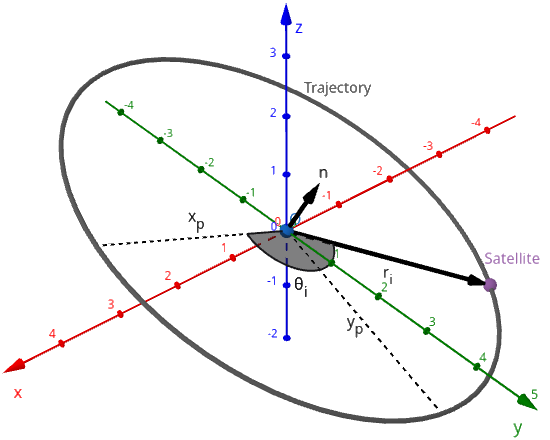
\includegraphics[width=0.43\linewidth]{images/radii_and_angles_in3d.png}
		\caption{The parametric trajectory in the three dimensional ECI coordinate system.}
		\label{fig:radii_angles_in_3d}
	\end{figure}
	\noindent
	Illustrated above is a trajectory in three dimensions. It still resides completely within a two dimensional plane which is characterized solely by an orthonormal vector $n$ as the origin of the coordinate system always lies within the plane. Positions in this context are also referred to as $r_i$ with the difference being that they are vectors. The definition of angles $\theta_i$ is slightly more complex. Both $x_p$ and $y_p$ are defined as projected unit vectors $x_0=(1, 0, 0)$ and $y_0 = (0, 1, 0)$ in the orbital plane. For visual purposes their lengths are not properly represented.\newline
	The parametric model relies on $\theta_i$ lying in the range of $0 \leq \theta_i \leq 2\pi$ or $-\pi \leq \theta_i \leq \pi$ which can not be calculated using $\arccos(x)$ of the scalar product of two vectors. A more suitable trigonometric function is $\atantwo(y,x)$ as it can determine an angle in the range of $-\pi \leq \theta \leq \pi$ in the correct quadrant as the sign of both inputs is known \cite{python_atan2}. With these aspects a formula for $\theta_i$ can be derived. We start off with the definitions of $x_p$ and $y_p$:
	
	\begin{equation}
		\begin{aligned}
			x_p=n\times x_0 \\
			y_p=n\times y_0
		\end{aligned}
	\end{equation}
	These projected vectors can be seen as X- and Y-axis for the two dimensional parametric model. Next up, apply scalar products to $r_i$ to determine its fractions $x$ and $y$ relative to $x_p$ and $y_p$:
	\begin{equation}
		\begin{aligned}
			x=r_i\cdot x_p \\
			y=r_i\cdot y_p
		\end{aligned}
	\end{equation}
	With $\theta_i = \atantwo(y, x)$ we construct the following formula
	\begin{equation}
		\label{theta_3d}
		\boxed{\theta_i=\atantwo(r_i\cdot(n\times x_0), r_i\cdot(n\times y_0))}
	\end{equation}
	which satisfies the requirement of $-\pi \leq \theta_i \leq \pi$. Henceforth, this adapion makes the parametric model usable in a three dimensional environment, as angles and magnitudes can now be determined from vectors for the two dimensional model.\newline
	Lastly, a method for determining the orthonormal plane vector $n$ has to be established. A measurement series of satellite positions $r_1, r_2, r_3,..., r_n$ may contain numerous entries. It must contain at least two entries so that the cross product between two vectors can be formed as follows:
	\begin{equation}
		\label{normal_plane}
		\boxed{n=\frac{r_i\times r_j}{|r_i|\cdot|r_j|}}
	\end{equation}
	\noindent
	In principle, all vectors of a series should lie exactly within the plane, such that it should not matter which two vectors get chosen to form the cross product. Due to measurement errors caused by various factors this may not be the case. Only the two vectors spanning the plane will fit perfectly, whereas the others might deviate slightly.
	
	\subsection{Orbit determination with two cameras}
	\label{sec:orbit_two_cameras}
	The previous two sections have established models under the assumption that $r_i$ vectors are readily available for computation but as of yet we have no methods for determining them. The only vectors which are readily available are position vectors $p_i$ and view vectors $v_i$. One approach for determining satellite positions is to use a two camera setup as illustrated below:
	
	\begin{figure}[H]
		\centering
		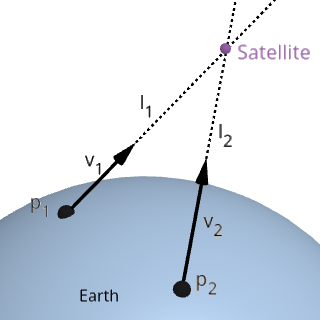
\includegraphics[width=0.4\linewidth]{images/stereo_vision.png}
		\caption{The parametric trajectory in the three dimensional ECI coordinate system.}
		\label{fig:two_camera_sat_pos_determination}
	\end{figure}
	\noindent
	Hereby, two cameras in different locations take an image of the satellite simultaneously. Immediatly known are their position- and view vectors. These properties form two lines $l_1$ and $l_2$ defined as
	
	\begin{equation}
		\begin{aligned}
			l_1(t) = p_1 +t\cdot v_1 \quad t \in \mathbb{R} \\
			l_2(s) = p_2 +s\cdot v_2 \quad s \in \mathbb{R}
		\end{aligned}
	\end{equation}
	\noindent
	which should intersect each other in a mathematical setting. However in a physical setting where cameras are limited in accuracy an exact intersection is unlikely to occur. A feasible guess for satellite location would be the closest approach between the two lines, more specifically the point in the middle of $l_1$ and $l_2$ where they approach each other the closest. \newline
	Fitzpatrick presents a readily available solution. At their points of closest approach $l_2(s)-l_1(t)$ is minimal in magnitude and perpendicular both to $v_1$ and $v_2$ meaning that scalar products between view vectors and $l_2(s)-l_1(t)$ should be zero:
	\begin{equation}
		\label{sysm_of_linear_eqs}
		\begin{aligned}
			0=v_1\cdot(l_2(s)-l_1(t)) \\
			0=v_2\cdot(l_2(s)-l_1(t))
		\end{aligned}
	\end{equation}
	This expression can be rearranged into a system of linear equations yielding solutions for $t$ and $s$ hereby defined as $t_{min}$ and $s_{min}$ where the distance between the lines is at their minimum.\cite{lines_closest_approach}\newline
	As there is no intersection the satellite position $r_i$ can not be determined exactly. However as feasible value we define $r_i $ as the point located in the middle between $l_1$ and $l_2$ at their minimum distance as follows:
	\begin{equation}
		\label{sat_position_2cams}
		\boxed{r_i = l_1(t_{min})+\frac{1}{2}(l_2(s_{min})-l_1(t_{min}))}
	\end{equation}
	Thereby, we obtain a method for full orbit determination using two cameras which can be formulated as a process:
	
	\begin{enumerate}
		\item Measure position vectors $p_i$ and $v_i$ of two observing cameras for three points in time resulting in six measured vectors total.
		\item Determine three radii vectors $r_1$, $r_2$ and $r_3$ using equation \ref{sat_position_2cams}. The system of linear equations resulting from expression \ref{sysm_of_linear_eqs} needs to be solved beforehand to obtain $t_{min}$ and $s_{min}$ for each observation.
		\item Chose two radii vectors and determine the plane normal vector $n$ using equation \ref{normal_plane}.
		\item With $n$ established, determine the angle $\theta_i$ for each radii vecto $r_i$ using equation \ref{theta_3d}.
		\item The values of $r_i$ will now be referred to as magnitudes of their corresponging radii vectors. Magnitudes $r_i$ and angles $\theta_i$ serve as input for the process defined in section \ref{sec:parametric_trajectory} which yields a parametric model.\newline \textbf{Done.}
	\end{enumerate}
	
	
	\subsection{Gaussian method of orbit determination}
	The Gaussian method of orbit determination is an algorithm originally developed by Gauss that requires only a single camera, thus a less complex setup than the previous approach.\newline
	Curtis provides the complete algorithm, as in the initial idea, the derivation and the final process which can be used for computation. In the following, we are only going have a look at the idea and the process as the derivation of underlying equations is of no particular relevance for the scope. Furthermore, we are going to apply some modifications to the process, as we can use some previously established solutions to reduce the number of steps. We start off with geometric context and the initial idea, illustrated in the figure below:
	
	\begin{figure}[H]
		\centering
		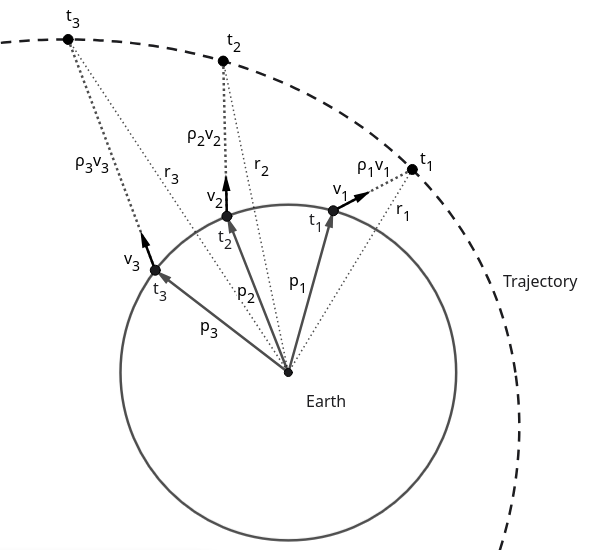
\includegraphics[width=0.6\linewidth]{images/gauss_known_and_unknown.png}
		\caption{Initially known and unknown properties of Gaussian orbit determination depicted in a two dimensional represention.}
		\label{fig:gauss_algo_idea}
	\end{figure}
	\noindent
	Initially, three observations at three different time stamps $t_1$, $t_2$ and $t_3$ from a fixed location on earth are taken, which yield three position vectors $p_1$, $p_2$ and $p_3$ as well as three view vectors $v_1$, $v_2$ and $v_3$. Unknown vectors are the satellite positions or radii vectors $r_1$, $r_2$ and $r_3$ similar to section \ref{sec:eath_bound_observation}. They can be described using the following relations
	
	\begin{equation}
		\label{gauss_algo_r_vectors}
		r_1=p_1+\rho_1v_1 \qquad r_2=p_2+\rho_2v_2 \qquad r_3=p_3+\rho_3v_3
	\end{equation}
	\noindent
	with $\rho_i \in \mathbb{R}$ for $i \in \{1,2,3\}$. Through this we reduce the unknown parameters to three real numbers. The goal of this algorithm is to determine fitting solutions for the unknowns so that the observations match a physical orbit around planet earth considering gravitational parameters. This solution can be calculated using the following procedure as elaborated by Curtis:
	
	\begin{enumerate}
		\item Determine time intervals $\tau_1$, $\tau_3$ and $\tau$ from $t_1$, $t_2$ and $t_3$ as follows: 
		\begin{equation}
			\tau_1 = t_1 - t_2 \qquad \tau_3 = t_3 - t_2 \qquad \tau = \tau_3 -\tau_1
		\end{equation}
		
		\item Determine the cross products $m_1$, $m_2$ and $m_3$ from view vectors $v_1$, $v_2$ and $v_3$ as follows:
		\begin{equation}
			m_1=v_2\times v_3 \qquad m_2=v_1\times v_3 \qquad m_3=v_1\times v_2
		\end{equation}
		
		\item Determine the scalar product $D_0$ as follows:
		\begin{equation}
			D_0=v_1\cdot m_1
		\end{equation}
		
		\item Calculate the nine scalar products $D_{ij}$ for $i,j \in \{1,2,3\}$ as follows:
		\begin{equation}
			\begin{aligned}
				D_{11}=p_1\cdot m_1 \qquad D_{12}=p_1\cdot m_2 \qquad D_{13}=p_1\cdot m_3 \\
				D_{21}=p_2\cdot m_1 \qquad D_{22}=p_2\cdot m_2 \qquad D_{23}=p_2\cdot m_3 \\
				D_{31}=p_3\cdot m_1 \qquad D_{32}=p_3\cdot m_2 \qquad D_{33}=p_3\cdot m_3
			\end{aligned}
		\end{equation}
		
		\item Calculate real number parameters $A$ and $B$ with the following expressions:
		\begin{equation}
			\begin{aligned}
				A = \frac{1}{D_0}
				\left(
				-D_{12}\frac{\tau_3}{\tau}
				+ D_{22}
				+ D_{32}\frac{\tau_1}{\tau}
				\right) \\
				B = \frac{1}{6D_0}
				\left(
				D_{12}\left(\tau_3^2-\tau^2\right)\frac{\tau_3}{\tau}
				+
				D_{32}\left(\tau^2-\tau_1^2\right)\frac{\tau_1}{\tau}
				\right)
			\end{aligned}
		\end{equation}
		
		\item Determine the scalar products $E$ and $p_2^2$ as follows:
		\begin{equation}
			E=p_2 \cdot v_2 \qquad p_2^2=p_2\cdot p_2
		\end{equation}
		
		\item Determine the real number parameters $a$, $b$ and $c$ with the following expressions:
		\begin{equation}
			\begin{aligned}
				a = -\left(A^2 + 2AE + p_2^2\right) \qquad b = -2\mu B(A + E) \qquad c = -\mu^2 B^2
			\end{aligned}
		\end{equation}
		\noindent
		Hereby, $\mu$ represents the gravitational parameter, the product of earth's mass and the universal gravity constant.
		
		\item An eighth degree polynomial equation containing the parameters $a$, $b$ and $c$ is defined as follows:
		\begin{equation}
			x^8+ax^6+bx^3+c=0
		\end{equation}
		\noindent
		Of this polynomial, a real number root $w$ larger than zero as solution for $x$  must be determined. If there is more than one solution $w$ it means that there is more than one physically feasible trajectory. The entire algorithm must be started over from step 1 exchanging one of the measurements for an additional one until a signle solution $w$ has been determined. For computation, Curtis proposes using Newton's method and plotting the polynomial as function to determine a proper initial estimate of $x$. We propose using a solver like NumPy roots which determines the roots of any polynomial \cite{numpy_roots} and works out of the box.
		
		\item Determine the unknown parameters $\rho_1$, $\rho_2$ and $\rho_3$ using $w$ with the following expressions:
		\begin{equation}
			\begin{aligned}
				\rho_1 =
				\frac{1}{D_0}
				\left(
				\frac{
					6\left(
					D_{31}\frac{\tau_1}{\tau_3}
					+
					D_{21}\frac{\tau}{\tau_3}
					\right)w^3
					+
					\mu D_{31}
					\left(\tau^2-\tau_1^2\right)
					\frac{\tau_1}{\tau_3}
				}{
					6w^3+\mu\left(\tau^2-\tau_3^2\right)
				}
				-
				D_{11}
				\right) \\
				\rho_3 =
				\frac{1}{D_0}
				\left(
				\frac{
					6\left(
					D_{13}\frac{\tau_3}{\tau_1}
					-
					D_{23}\frac{\tau}{\tau_1}
					\right)w^3
					+
					\mu D_{13}
					\left(\tau^2-\tau_3^2\right)
					\frac{\tau_3}{\tau_1}
				}{
					6w^3+\mu\left(\tau^2-\tau_1^2\right)
				}
				-
				D_{33}
				\right) \\
				\rho_2 = A + \frac{\mu B}{w^3} 
			\end{aligned}
		\end{equation}
		
		\item Use the previously defined equations \ref{gauss_algo_r_vectors} to determine $r_1$, $r_2$ and $r_3$ from $\rho_1$, $\rho_2$ and $\rho_3$ and already known vectors.
	\end{enumerate}
	\cite{curtis_gauss_algo}
	\newline
	From here on onwards the Gauss algorithm as presented by Curtis contains three additional steps to establish orbital properties from $r_1$, $r_2$ and $r_3$ determined in step 10. However, we have already established a method to determine orbital properties which we reuse to formulate a sigle final step as follows:
	
	\begin{enumerate}
		\setcounter{enumi}{10}
		\item Use the orbit determination procedure established in section \ref{sec:orbit_two_cameras} starting from step 3 as $r_1$, $r_2$ and $r_3$ are already known. This yields vector $n$ and a parametric model.\newline
		\textbf{Done.}
	\end{enumerate}
	
	
	
	\subsection{Simplified Gaussian method of orbit determination}
	The previously presented Gaussian method determines viable parameters to form all types of parametric trajectories that fit observations to physical orbits. Due to orbits of satellites at lower altitudes above the earth being mostly circular we propose a method that always assumes a circular model. This way we only need to determine the plane normal vector $n$ and the semi major axis $a$. The aspect that we want to keep is the use of a single camera so that the setup is very much similar to figure \ref{fig:gauss_algo_idea}, except that one measurement less is needed. Known values are the position vectors $p_1$, $p_2$, the view vectors $v_1$, $v_2$, whereupon they are related similar to expression \ref{gauss_algo_r_vectors} so that $r_1$, $r_2$, $\rho_1$ and $\rho_2$ are unknowns. Furthermore, the time stamps $t_1$, $t_2$ of measurement recordings are supposed to be known.\newline
	We start off with the circularity condition, meaning that all radii vectors $r_i$ must posess the same magnitude which formulates as follows: 
	\begin{equation}
		\label{circle_gauss_circle_condition}
		\boxed{|r_1|=|r_2|\Leftrightarrow \sqrt{(p_1+\rho_1v_1)^2}=\sqrt{(p_2+\rho_2v_2)^2}}
	\end{equation}
	\noindent
	Next, the orbital period $T$ subject to the semi major axis $a$ and the gravitational parameter $\mu$ can be expressed as follows:
	\begin{equation}
		\label{circle_gauss_period}
		T=\frac{2\pi}{\sqrt{\mu}}a^{\frac{3}{2}}=\frac{2\pi}{\sqrt{\mu}}|r_i|^{\frac{3}{2}}
	\end{equation}
	\cite{elliptical_orbits}\newline
	Knowing that $a=|r_1|=|r_2|$, the value of $a$ can be substituted for the magnitude of any radius vector $r_i$. Next, the angle $\varphi$ with $0 \leq \varphi \leq \pi$ between $r_1$ and $r_2$ can be described using the $\arccos$ as follows:
	\begin{equation}
		\label{circle_gauss_phi}
		\varphi = \arccos\left(\frac{r_1\cdot r_2}{|r_1|\cdot|r_2|}\right)
	\end{equation}
	\noindent
	This angle describes the arc of the circlular orbit which the satellite traverses between time stamps $t_1$ and $t_2$ under the condition that $t_2 - t_1 \leq \frac{T}{2}$. This restriction needs to be in place, because the output range of $\arccos$ does not cover a full circle. This relation between time stamps and arc formulates as:
	\begin{equation}
		\label{circle_gauss_delta_t}
		t_2 - t_1 = \Delta t=\frac{\varphi}{2\pi}T
	\end{equation}
	\noindent
	Equations \ref{circle_gauss_period} and \ref{circle_gauss_phi} can be inserted into $\ref{circle_gauss_delta_t}$ to form the following expression
	
	\begin{equation*}
		\begin{aligned}
			\frac{\arccos\left(\frac{r_1\cdot r_2}{|r_1|\cdot|r_2|}\right)}{2\pi}\cdot
			\frac{2\pi}{\sqrt{\mu}}|r_1|^{\frac{3}{2}}=
			\Delta t \Leftrightarrow \\
			\arccos\left(\frac{r_1\cdot r_2}{|r_1|^2}\right)\cdot|r_1|^{\frac{3}{2}}=\Delta t\sqrt{\mu}
		\end{aligned}
	\end{equation*}
	which yields the time condition subject to $\rho_1$ and $\rho_2$ formulated as:
	\begin{equation}
		\label{circle_gauss_time_condition}
		\boxed{\arccos\left(\frac{(p_1+\rho_1v_1)\cdot (p_2+\rho_2v_2)}{|(p_1+\rho_1v_1)|^2}\right)\cdot|(p_1+\rho_1v_1)|^{\frac{3}{2}}=(t_2-t_1)\sqrt{\mu}}
	\end{equation}
	\noindent
	With cirularity and time conditions established we can formulate a full orbit determination process as follows:
	
	\begin{enumerate}
		\item Measure position vectors $p_1$, $p_2$ and view vectors $v_1$, $v_2$ of two time stamps $t_1$ and $t_2$. A crucial requirement for this algorithm to work is that $t_2 - t_1 \leq \frac{T}{2}$ meaning that observation arcs can not take longer than half the orbital period.
		\item A real number solution for $\rho_1$ and $\rho_2$ must be computed which satifies the time condition \ref{circle_gauss_time_condition} constrained by the circularity condition \ref{circle_gauss_circle_condition}. This task can not be acomplished analytically. For this reason we propose the use of a sophisticated solver like scipy.optimize.root which allows for modeling more complex functions to be solved numerically \cite{scipy_roots}. This yields the two values $\rho_1$ and $\rho_2$.
		\item Calculate $r_1$ and $r_2$ using expressions \ref{gauss_algo_r_vectors}. Obtain the plane normal vector $n$ using equation \ref{normal_plane}. The semi major axis $a$ equates radii vector magnitudes $a=|r_1|=|r_2|$.\newline
		\textbf{Done.}
	\end{enumerate}
	\newpage
	
	
	\begin{thebibliography}{9}
		\setlength{\itemsep}{4pt}       % space between bibliography items
		\setlength{\parskip}{0pt}       % space between paragraphs
		\setlength{\parsep}{0pt}        % extra space within items
		
		\bibitem{orbit_equation}
		Orbital Mechanics \& Astrodynamics \emph{The Orbit Equation}, Bryan Weber, \url{https://orbital-mechanics.space/the-orbit-equation/the-orbit-equation.html}. \newline Accessed 09.08.2026
		
		\bibitem{orbital_nomenclature}
		Orbital Mechanics \& Astrodynamics \emph{Orbital Nomenclature}, Bryan Weber, \url{https://orbital-mechanics.space/the-orbit-equation/orbital-nomenclature.html}. \newline Accessed 09.08.2026
		
		\bibitem{elliptical_orbits}
		Orbital Mechanics \& Astrodynamics \emph{Elliptical Orbits}, Bryan Weber, \url{https://orbital-mechanics.space/the-orbit-equation/elliptical-orbits.html}. \newline Accessed 09.08.2026
		
		\bibitem{hyperbolic_orbits}
		Orbital Mechanics \& Astrodynamics \emph{Hyperbolic Trajectories}, Bryan Weber, \url{https://orbital-mechanics.space/the-orbit-equation/hyperbolic-trajectories.html}. \newline Accessed 09.08.2026
		
		\bibitem{parabolic_orbits}
		Orbital Mechanics \& Astrodynamics \emph{Parabolic Trajectories}, Bryan Weber, \url{https://orbital-mechanics.space/the-orbit-equation/parabolic-trajectories.html}. \newline Accessed 09.08.2026
		
		\bibitem{reference_frames}
		Orbital Mechanics \& Astrodynamics \emph{Reference Frames}, Bryan Weber, \url{https://orbital-mechanics.space/intro/reference-frames.html}. \newline Accessed 09.08.2026
		
		\bibitem{satellites_at_night}
		Can You See Satellites At Night? How Do You Spot Them?, 	Visnja Radosavljevic, Optics Mag, 2025, \url{https://opticsmag.com/can-you-see-satellites-at-night/}. \newline Accessed 13.08.2026
		
		\bibitem{esa_cartesian_ellipsoidal}
		J. Sanz Subirana, J.M. Juan Zornoza and M. Hernández-Pajares, "Coordinate Conversions", Gnss Data Processing Volume I: Fundamentals and Algorithms, 2013, p. 185, \url{https://gssc.esa.int/navipedia/GNSS_Book/ESA_GNSS-Book_TM-23_Vol_I.pdf}. \newline Accessed 14.08.2026
		
		\bibitem{curtis_siderial_time}
		H.D. Curtis, "Siderial Time", Orbital Mechanics for Engineering Students 2nd Edition, 2010, pp. 275-280, \url{https://shop.elsevier.com/books/orbital-mechanics-for-engineering-students/curtis/978-0-12-374778-5}\newline
		Accessed 03.05.2026
		
		\bibitem{self_localization_in_space}
		Frederic Heil "Determining attitude to the background stars", \emph{Image based self localization in interplanetary space}, 2025, pp. 9-11,\newline \url{https://github.com/stonkchonk/satellite-trajectories/blob/main/thesis/papers/heil_self_localization_2025.pdf}\newline
		Accessed 23.08.2026
		
		\bibitem{four_stars_algo}
		Dong Ying, Xing Fei, You Zheng. Brightness Independent 4-Star Matching Algorithm
		for Lost-in-Space 3-Axis Attitude Acquisition, 2006,\newline
		\url{https://www.sciencedirect.com/science/article/abs/pii/S1007021406702322}\newline
		Accessed 23.08.2026
		
		\bibitem{python_atan2}
		"Trigonometric functions" The Python Standard Library, 2026,\newline
		\url{https://docs.python.org/3/library/math.html#math.atan2}\newline
		Accessed 28.08.2026
		
		\bibitem{lines_closest_approach}
		Sean Fitzpatrick, "Finding the closest points on skew lines." Elementary Linear Algebra: For University of Lethbridge Math 1410, \newline
		\url{https://opentext.uleth.ca/Math1410/sec-lines.html}\newline
		Accessed 29.08.2026
		
		\bibitem{curtis_gauss_algo}
		H.D. Curtis, "Gauss method of preliminary orbit determination", Orbital Mechanics for Engineering Students 2nd Edition, 2010, pp. 297-304, \url{https://shop.elsevier.com/books/orbital-mechanics-for-engineering-students/curtis/978-0-12-374778-5}\newline
		Accessed 03.05.2026
		
		\bibitem{numpy_roots}
		"numpy.roots" NumPy documentation, 2026,\newline
		\url{https://numpy.org/doc/stable/reference/generated/numpy.roots.html}\newline
		Accessed 30.08.2026
		
		\bibitem{scipy_roots}
		"scipy.optimize.root" SciPy documentation, 2026,\newline
		\url{https://docs.scipy.org/doc/scipy/reference/generated/scipy.optimize.root.html}\newline
		Accessed 30.08.2026
		
	\end{thebibliography}
\end{document}